\begin{enumerate}[label=\thesubsection.\arabic*, ref=\thesubsection.\theenumi]
\item For given vectors,  $\vec{a}=2\hat{i}-\hat{j}+2\hat{k}$ and $\vec{b}=-\hat{i}+\hat{j}-\hat{k}$ ,  find the unit vector in the
direction of the vector $\vec{a}+\vec{b}$.
        \label{prob:12/10/2/9}
\\
    \solution 
		Let 
\begin{align}
	\vec{a} = \myvec{1\\1\\1} , \vec{b} = \myvec{2\\ -7 \\ -3}, 
\vec{c} = \myvec{\dfrac{1}{\sqrt{3}}\\[2ex] \dfrac{1}{\sqrt{3}} \\[2ex] -\dfrac{1}{\sqrt{3}}} 
\label{eq:chapters/12/10/2/1/1}
\end{align}
Then
\begin{align}
	{\vec{a}^{\top}\vec{a}} &= \myvec{1  &  1  &  1}\myvec{1\\1\\1} = 3
\\
\implies 
	\norm{\vec{a}}&=\sqrt{3}, 
	\label{eq:chapters/12/10/2/1/3}
\end{align}
		from \eqref{eq:side-length}. Similarly,
\begin{align}
	\norm{\vec{b}}&=\sqrt{\vec{b}^{\top}\vec{b}}= \sqrt{62}, 
	\label{eq:chapters/12/10/2/1/4}
	\\ \norm{\vec{c}}&=\sqrt{\vec{c}^{\top}\vec{c}}	
=1
	\label{eq:chapters/12/10/2/1/5}
\end{align}




\item Find the unit vector in the direction of sum of vectors $\vec{a}$= $2\hat{i}-\hat{j}+\hat{k}$  and  $\vec{b}=2\hat{j}+\hat{k}$.
\item If $\vec{a}$=$\hat{i}+\hat{j}+2\hat{k}$  and  $\vec{b}$=$2\hat{i}+\hat{j}-2\hat{k}$,  find the unit vector in the direction of
	\begin{enumerate}
		\item 6$\vec{a}$   
		\item 2$\vec{a}$-$\vec{b}$
	\end{enumerate}

\item Find the value of $x$ for which $x(\hat{i}+\hat{j}+\hat{k})$ is a unit vector.\\
	\solution
		Let 
\begin{align}
	\vec{a} = \myvec{1\\1\\1} , \vec{b} = \myvec{2\\ -7 \\ -3}, 
\vec{c} = \myvec{\dfrac{1}{\sqrt{3}}\\[2ex] \dfrac{1}{\sqrt{3}} \\[2ex] -\dfrac{1}{\sqrt{3}}} 
\label{eq:chapters/12/10/2/1/1}
\end{align}
Then
\begin{align}
	{\vec{a}^{\top}\vec{a}} &= \myvec{1  &  1  &  1}\myvec{1\\1\\1} = 3
\\
\implies 
	\norm{\vec{a}}&=\sqrt{3}, 
	\label{eq:chapters/12/10/2/1/3}
\end{align}
		from \eqref{eq:side-length}. Similarly,
\begin{align}
	\norm{\vec{b}}&=\sqrt{\vec{b}^{\top}\vec{b}}= \sqrt{62}, 
	\label{eq:chapters/12/10/2/1/4}
	\\ \norm{\vec{c}}&=\sqrt{\vec{c}^{\top}\vec{c}}	
=1
	\label{eq:chapters/12/10/2/1/5}
\end{align}




\item Find a vector in the direction of vector $5\hat{i}-\hat{j}+2\hat{k}$ which has magnitude 8 units.
        \label{prob:12/10/2/10const}
   \\ 
    \solution 
		Let 
\begin{align}
	\vec{a} = \myvec{1\\1\\1} , \vec{b} = \myvec{2\\ -7 \\ -3}, 
\vec{c} = \myvec{\dfrac{1}{\sqrt{3}}\\[2ex] \dfrac{1}{\sqrt{3}} \\[2ex] -\dfrac{1}{\sqrt{3}}} 
\label{eq:chapters/12/10/2/1/1}
\end{align}
Then
\begin{align}
	{\vec{a}^{\top}\vec{a}} &= \myvec{1  &  1  &  1}\myvec{1\\1\\1} = 3
\\
\implies 
	\norm{\vec{a}}&=\sqrt{3}, 
	\label{eq:chapters/12/10/2/1/3}
\end{align}
		from \eqref{eq:side-length}. Similarly,
\begin{align}
	\norm{\vec{b}}&=\sqrt{\vec{b}^{\top}\vec{b}}= \sqrt{62}, 
	\label{eq:chapters/12/10/2/1/4}
	\\ \norm{\vec{c}}&=\sqrt{\vec{c}^{\top}\vec{c}}	
=1
	\label{eq:chapters/12/10/2/1/5}
\end{align}




	\item 
Find a vector of magnitude 5 units,  and parallel to the resultant of the vectors $\vec{a} = 2\hat{i}+3\hat{j}-\hat{k}$ and $\vec{b} = \hat{i}-2\hat{j}+\hat{k}$.
\\
\solution
		\input{chapters/12/10/5/6/asgnt2.tex}
\item Find a unit vector in the direction of $\overline{PQ} $,  where $\vec{P}$ and $\vec{Q}$ have co-ordinates (5, 0, 8) and (3, 3, 2), respectively.
\item Find the unit vector in the direction of the vector $\vec{a}=\hat{i}+\hat{j}+2\hat{k}$.
\item Find the unit vector in the direction of vector $\overrightarrow{PQ}$ ,  where $\vec{P}$ and $\vec{Q}$ are the points
(1,  2,  3) and (4,  5,  6),  respectively.
\item The vector in the direction of the vector $\hat{i}-2\hat{j}+2\hat{k}$ that has magnitude 9 is
	\begin{enumerate}
\item $\hat{i}-2\hat{j}+2\hat{k}$
\item $\hat{i}-2\hat{j}$
\item $3(\hat{i}-2\hat{j}+2\hat{k})$
\item $9(\hat{i}-2\hat{j}+2\hat{k})$
\end{enumerate}
\item Find a vector of magnitude 5 units,  and parallel to the resultant of the vectors $\vec{a}=2\hat{i}+3\hat{j}-\hat{k}$ and $\vec{b}=\hat{i}-2\hat{j}+\hat{k}$.\\
\item If $\vec{a}=\hat{i}+\hat{j}+\hat{k},  \vec{b}=2\hat{i}-\hat{j}+3\hat{k}$ and $\vec{c}=\hat{i}-2\hat{j}+\hat{k}$,  find a unit vector parallel to the vector $2\vec{a}-\vec{b}+3\vec{c}$.\\
	\solution
		Let 
\begin{align}
	\vec{a} = \myvec{1\\1\\1} , \vec{b} = \myvec{2\\ -7 \\ -3}, 
\vec{c} = \myvec{\dfrac{1}{\sqrt{3}}\\[2ex] \dfrac{1}{\sqrt{3}} \\[2ex] -\dfrac{1}{\sqrt{3}}} 
\label{eq:chapters/12/10/2/1/1}
\end{align}
Then
\begin{align}
	{\vec{a}^{\top}\vec{a}} &= \myvec{1  &  1  &  1}\myvec{1\\1\\1} = 3
\\
\implies 
	\norm{\vec{a}}&=\sqrt{3}, 
	\label{eq:chapters/12/10/2/1/3}
\end{align}
		from \eqref{eq:side-length}. Similarly,
\begin{align}
	\norm{\vec{b}}&=\sqrt{\vec{b}^{\top}\vec{b}}= \sqrt{62}, 
	\label{eq:chapters/12/10/2/1/4}
	\\ \norm{\vec{c}}&=\sqrt{\vec{c}^{\top}\vec{c}}	
=1
	\label{eq:chapters/12/10/2/1/5}
\end{align}




	\item If a line makes angles $90\degree, 135\degree, 45\degree$ with X, Y and Z axis respectivly. Find its direction cosines.
		\\
		\solution
		\input{chapters/12/11/1/1/vec.tex}
\item Find the direction cosines of the vector joining the points $\vec{A}$ (1,  2,  –3) and
$\vec{B}$(–1,  –2,  1),  directed from $\vec{A}$ to $\vec{B}$.
	\\
    \solution 
		Let 
\begin{align}
	\vec{a} = \myvec{1\\1\\1} , \vec{b} = \myvec{2\\ -7 \\ -3}, 
\vec{c} = \myvec{\dfrac{1}{\sqrt{3}}\\[2ex] \dfrac{1}{\sqrt{3}} \\[2ex] -\dfrac{1}{\sqrt{3}}} 
\label{eq:chapters/12/10/2/1/1}
\end{align}
Then
\begin{align}
	{\vec{a}^{\top}\vec{a}} &= \myvec{1  &  1  &  1}\myvec{1\\1\\1} = 3
\\
\implies 
	\norm{\vec{a}}&=\sqrt{3}, 
	\label{eq:chapters/12/10/2/1/3}
\end{align}
		from \eqref{eq:side-length}. Similarly,
\begin{align}
	\norm{\vec{b}}&=\sqrt{\vec{b}^{\top}\vec{b}}= \sqrt{62}, 
	\label{eq:chapters/12/10/2/1/4}
	\\ \norm{\vec{c}}&=\sqrt{\vec{c}^{\top}\vec{c}}	
=1
	\label{eq:chapters/12/10/2/1/5}
\end{align}




\item Show that the vector $\hat{i}+\hat{j}+\hat{k}$ is equally inclined to the axes OX,  OY and OZ.
	\\
\solution
		\solution 
See Fig. \ref{fig:10/7/4/8Fig3}. From 
  \eqref{eq:10/7/4/8det2f}, $PQRS$ is a parallelogram.
\begin{align}
  %\label{eq:10/7/4/8det2f}
  \vec{P}  = 
 \myvec{3 \\2},\, 
 \vec{Q}  = \myvec{
 2 \\
 4 \\
 } ,\,
 \vec{R}  = \myvec{
 5 \\
 \frac{3}{2}
 }   
  ,\,
 \vec{S}  = \myvec{
 2\\
 -1 \\
 }   
 \\
	\implies 
 \brak{\vec{Q}-\vec{P}}^\top\brak{\vec{R}-\vec{Q}}  \neq 0
 \\
 \brak{\vec{R}-\vec{P}}^\top\brak{\vec{S}-\vec{Q}}  = 0
\end{align}
Therefore $PQRS$ is a rhombus.
\begin{figure}[H]
	\begin{center}
		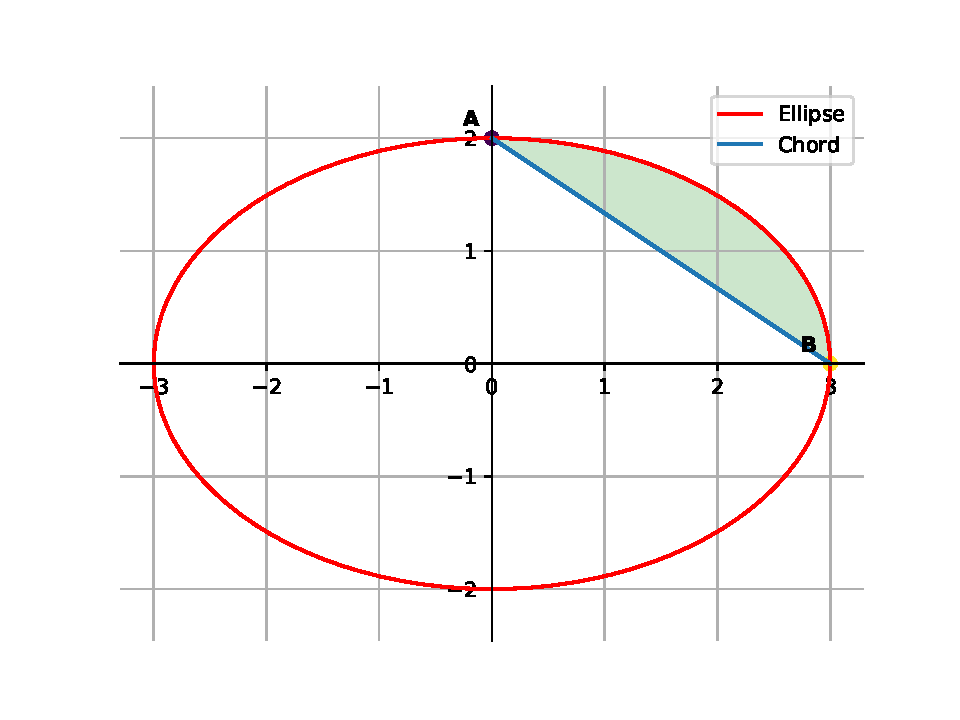
\includegraphics[width=0.75\columnwidth]{chapters/10/7/4/8/figs/fig.pdf}
	\end{center}
\caption{}
\label{fig:10/7/4/8Fig3}
\end{figure}


\item Find the unit vector in the direction of vector $\overrightarrow{a} = 2\hat{i} +3\hat{j} +\hat{k}$.
\item Find the unit vector in the direction of the sum of the vectors, $\overrightarrow{a} = 2\hat{i} +2\hat{j} -5\hat{k}$ and $\overrightarrow{b} = 2\hat{i} +\hat{j} +3\hat{k}$.
\item Write the direction ratios of the vector $\overrightarrow{a} = \hat{i} +\hat{j} -\hat{k}$ and hence calculate its direction cosines.
\item If a line has direction ratios $2, -1, -2$, determine its direction cosines.
\item Find the direction cosines of the line passing through the two points $(-2, 4, -5)$ and $(1, 2, 3)$.
\item If a line has the direction ratios –18,  12,  –4,  then what are its direction cosines?
		\\
		\solution
		Let 
\begin{align}
	\vec{a} = \myvec{1\\1\\1} , \vec{b} = \myvec{2\\ -7 \\ -3}, 
\vec{c} = \myvec{\dfrac{1}{\sqrt{3}}\\[2ex] \dfrac{1}{\sqrt{3}} \\[2ex] -\dfrac{1}{\sqrt{3}}} 
\label{eq:chapters/12/10/2/1/1}
\end{align}
Then
\begin{align}
	{\vec{a}^{\top}\vec{a}} &= \myvec{1  &  1  &  1}\myvec{1\\1\\1} = 3
\\
\implies 
	\norm{\vec{a}}&=\sqrt{3}, 
	\label{eq:chapters/12/10/2/1/3}
\end{align}
		from \eqref{eq:side-length}. Similarly,
\begin{align}
	\norm{\vec{b}}&=\sqrt{\vec{b}^{\top}\vec{b}}= \sqrt{62}, 
	\label{eq:chapters/12/10/2/1/4}
	\\ \norm{\vec{c}}&=\sqrt{\vec{c}^{\top}\vec{c}}	
=1
	\label{eq:chapters/12/10/2/1/5}
\end{align}




	\item Find the direction cosines of the sides of a triangle whose vertices are $\myvec{3\\ 5\\-4 }$,  $\myvec{ -1\\1 \\2 }$ and $\myvec{-5 \\-5 \\-2 }$.
		\\
		\solution
		\solution 
See Fig. \ref{fig:10/7/4/8Fig3}. From 
  \eqref{eq:10/7/4/8det2f}, $PQRS$ is a parallelogram.
\begin{align}
  %\label{eq:10/7/4/8det2f}
  \vec{P}  = 
 \myvec{3 \\2},\, 
 \vec{Q}  = \myvec{
 2 \\
 4 \\
 } ,\,
 \vec{R}  = \myvec{
 5 \\
 \frac{3}{2}
 }   
  ,\,
 \vec{S}  = \myvec{
 2\\
 -1 \\
 }   
 \\
	\implies 
 \brak{\vec{Q}-\vec{P}}^\top\brak{\vec{R}-\vec{Q}}  \neq 0
 \\
 \brak{\vec{R}-\vec{P}}^\top\brak{\vec{S}-\vec{Q}}  = 0
\end{align}
Therefore $PQRS$ is a rhombus.
\begin{figure}[H]
	\begin{center}
		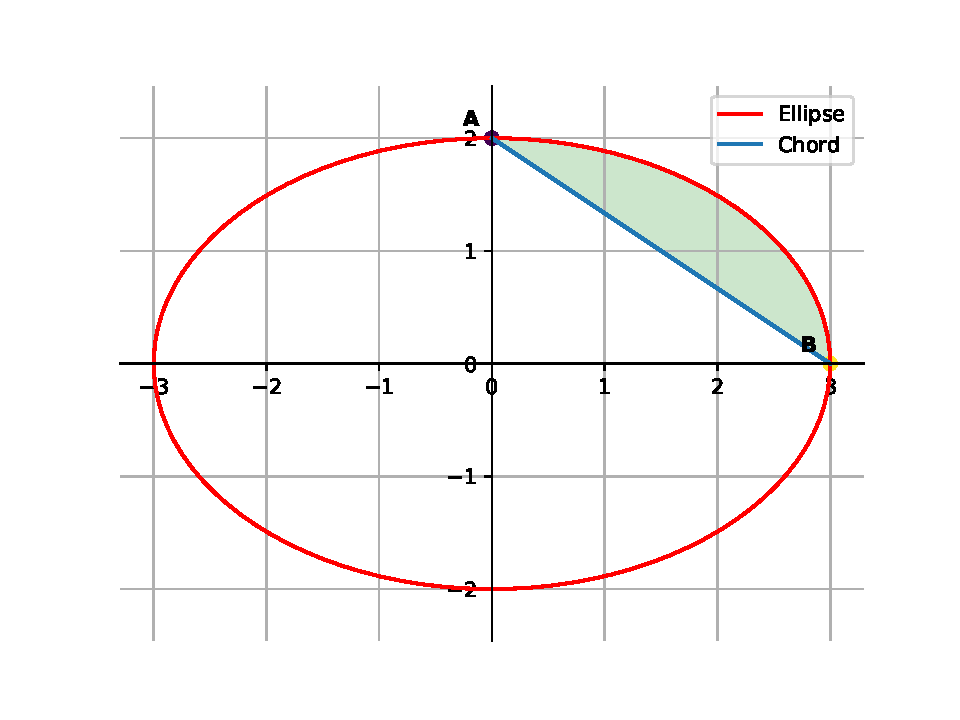
\includegraphics[width=0.75\columnwidth]{chapters/10/7/4/8/figs/fig.pdf}
	\end{center}
\caption{}
\label{fig:10/7/4/8Fig3}
\end{figure}


\item Find the direction cosines of the vector $\hat{i}+2\hat{j}+3\hat{k}$.
	\\
    \solution 
		\solution 
See Fig. \ref{fig:10/7/4/8Fig3}. From 
  \eqref{eq:10/7/4/8det2f}, $PQRS$ is a parallelogram.
\begin{align}
  %\label{eq:10/7/4/8det2f}
  \vec{P}  = 
 \myvec{3 \\2},\, 
 \vec{Q}  = \myvec{
 2 \\
 4 \\
 } ,\,
 \vec{R}  = \myvec{
 5 \\
 \frac{3}{2}
 }   
  ,\,
 \vec{S}  = \myvec{
 2\\
 -1 \\
 }   
 \\
	\implies 
 \brak{\vec{Q}-\vec{P}}^\top\brak{\vec{R}-\vec{Q}}  \neq 0
 \\
 \brak{\vec{R}-\vec{P}}^\top\brak{\vec{S}-\vec{Q}}  = 0
\end{align}
Therefore $PQRS$ is a rhombus.
\begin{figure}[H]
	\begin{center}
		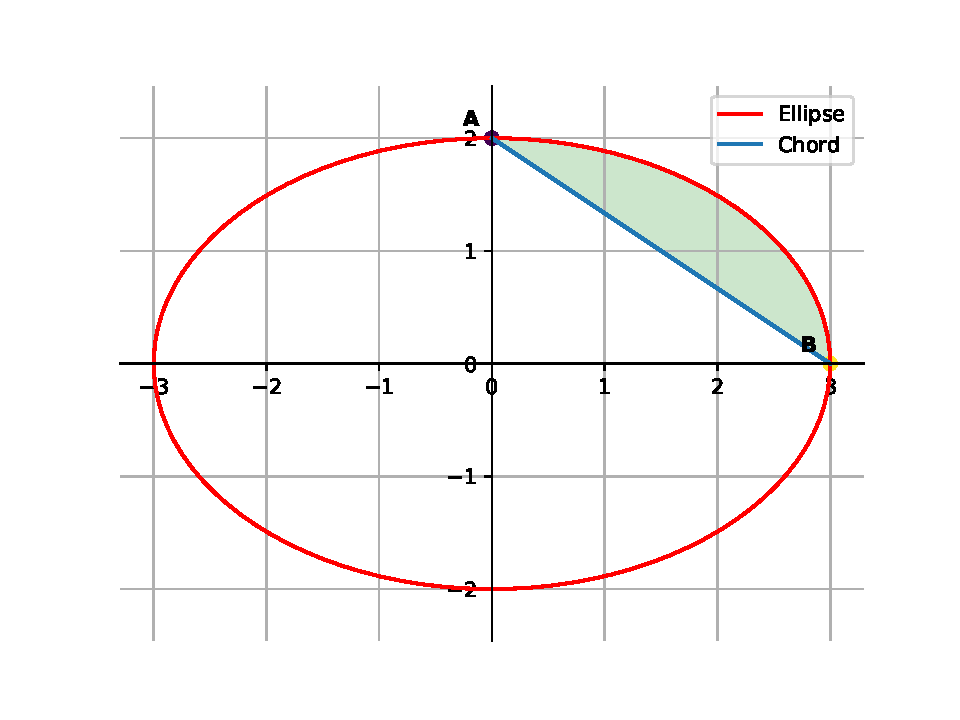
\includegraphics[width=0.75\columnwidth]{chapters/10/7/4/8/figs/fig.pdf}
	\end{center}
\caption{}
\label{fig:10/7/4/8Fig3}
\end{figure}


\item Find the direction cosines of the unit vector perpendicular to the plane $\overrightarrow{r} \cdot(6 \hat{i}- 3 \hat{j}- 2 \hat{k})+ 1= 0$ passing through the origin.
\item If a line makes angle $90 \degree, 60 \degree$ and $30 \degree$ with the positive direction of X, Y and Z axes respectively, find its direction cosines.
    \item Find the direction cosines of a line which makes equal angles with the coordinate
    axes.
		\\
		\solution
		Let 
\begin{align}
	\vec{a} = \myvec{1\\1\\1} , \vec{b} = \myvec{2\\ -7 \\ -3}, 
\vec{c} = \myvec{\dfrac{1}{\sqrt{3}}\\[2ex] \dfrac{1}{\sqrt{3}} \\[2ex] -\dfrac{1}{\sqrt{3}}} 
\label{eq:chapters/12/10/2/1/1}
\end{align}
Then
\begin{align}
	{\vec{a}^{\top}\vec{a}} &= \myvec{1  &  1  &  1}\myvec{1\\1\\1} = 3
\\
\implies 
	\norm{\vec{a}}&=\sqrt{3}, 
	\label{eq:chapters/12/10/2/1/3}
\end{align}
		from \eqref{eq:side-length}. Similarly,
\begin{align}
	\norm{\vec{b}}&=\sqrt{\vec{b}^{\top}\vec{b}}= \sqrt{62}, 
	\label{eq:chapters/12/10/2/1/4}
	\\ \norm{\vec{c}}&=\sqrt{\vec{c}^{\top}\vec{c}}	
=1
	\label{eq:chapters/12/10/2/1/5}
\end{align}




\item If a unit vector $\overrightarrow{a}$ makes angles $\frac{\pi}{3}\text{ with }\hat{i},  \frac{\pi}{4}\text{ with }\hat{j}$ and an acute angle $\theta \text{ with }\hat{k}, \text{ then find } \theta$ and hence,  the components of $\overrightarrow{a}$.
	\\
		\solution
		Let 
\begin{align}
	\vec{a} = \myvec{1\\1\\1} , \vec{b} = \myvec{2\\ -7 \\ -3}, 
\vec{c} = \myvec{\dfrac{1}{\sqrt{3}}\\[2ex] \dfrac{1}{\sqrt{3}} \\[2ex] -\dfrac{1}{\sqrt{3}}} 
\label{eq:chapters/12/10/2/1/1}
\end{align}
Then
\begin{align}
	{\vec{a}^{\top}\vec{a}} &= \myvec{1  &  1  &  1}\myvec{1\\1\\1} = 3
\\
\implies 
	\norm{\vec{a}}&=\sqrt{3}, 
	\label{eq:chapters/12/10/2/1/3}
\end{align}
		from \eqref{eq:side-length}. Similarly,
\begin{align}
	\norm{\vec{b}}&=\sqrt{\vec{b}^{\top}\vec{b}}= \sqrt{62}, 
	\label{eq:chapters/12/10/2/1/4}
	\\ \norm{\vec{c}}&=\sqrt{\vec{c}^{\top}\vec{c}}	
=1
	\label{eq:chapters/12/10/2/1/5}
\end{align}




\item Write down a unit vector in XY-plane,  making an angle of 30$\degree$ with the positive direction of X axis.\\
\item A vector $\vec{r}$ is inclined at equal angles to the three axis. If the magnitude of $\vec{r}$ is $2\sqrt{3}$ units,  find $\vec{r}$.
\item The direction cosines of the vector $(2\hat{i}+2\hat{j}-\hat{k})$ are \noindent\rule{2cm}{0.4pt}.
\item A vector $\vec{r}$ has a magnitude 14 and direction ratios 2,  3,  -6. Find the direction cosines and components of $\vec{r}$,  given that $\vec{r}$ makes an acute angle with X axis.
\end{enumerate}
